\section{Software}
\label{Sec:software}
Para que a aplicação Web possa receber os dados de consumo enviados pelo Módulo Coordenador, é necessário haver uma estrutura de rotas, métodos para lidar com objetos de classes, controladores e páginas de exibição para interagir com o usuário. Para isso, foi escolhida a arquitetura MVC, e um framework que consegue lidar com tal arquitetura. E para tornar a aplicação disponível para o acesso remoto através de smartphones, tablets e notebooks, optou-se por utilizar serviços de nuvem. 

\subsection{Tecnologia}

A seguir são apresentadas as tecnologias utilizadas para a implementação da aplicação Web.

\subsubsection{Django e Python}

O framework Django foi utilizado devido ao uso da linguagem python, que é uma linguagem limpa, de fácil utilização e com ampla disponibilidade de bibliotecas gratuitas e de fóruns para auxílio na implementação. Uma das vantagens do python nesse caso é a compatibilidade, pois o hardware foi construído com intenção de aprendizado através da linguagem de programação python \cite{raspberry_pi_site}(``pi'' em ``raspberry pi'' vem de ``python''). Outra vantagem é a experiência dos integrantes do grupo quanto ao manuseio do framework, o que agilizou o desenvolvimento. Outra vantagem é a possibilidade de utilizar, se necessário, o próprio raspberry como servidor da aplicação, bastando instalar as bibliotecas das dependências do Django.

O Django utiliza a arquitetura MVC. Os Models no Django contém os campos e os métodos dos objetos sendo utilizados. Todos as classes de Models herdam métodos e atributos da classe pré-existente Model do Django. Geralmente, cada Model é mapeado para uma tabela no banco de dados.

As Views (na arquitetura MVC) são chamadas Templates no Django. Elas são páginas no formato HTML que podem conter trechos de código em python para mostrar conteúdo do Context. Context é uma estrutura de chave-valor que provê o conteúdo a ser utilizado na página.

Os Controllers são chamados Views. O Django provê os chamados Base Views, que são classes que auxiliam a criação de Controllers. Podem ser utilizados diretamente, sobrescrevendo seus atributos e métodos, ou herdando estes para classes customizadas. Há três Base Views: 
\begin{description}
	\item[View:] É a classe a partir da qual se herdam todas as outras classes de Controllers.
	\item[TemplateView:] Renderiza um Template com um Context.
	\item[RedirectView:] Redireciona para uma dada URL.
\end{description} 

Outros Controllers pré-existentes são os Generic Display Views, que são Controllers genéricos utilizados normalmente para exibir dados de Models:
\begin{description}
	\item[DetailView:] Exibe detalhes um objeto.
	\item[ListView:] Exibe uma lista de objetos.
\end{description}

Há Controllers utilizados para edição de conteúdo, que são os Generic Editing Views:
\begin{description}
	\item[FormView:] Exibe um formulário e realiza validação e redirecionamento caso não haja erros.
	\item[CreateView:] Exibe um formulário para criação de objetos. Caso o formulário seja submetido e não haja erros na validação, cria o objeto.
	\item[UpdateView:] Exibe um formulário para edição de objetos. Caso o formulário seja submetido e não haja erros na validação, salva o objeto.
	\item[DeleteView:] Exibe uma página com uma caixa de confirmação para deletar um objeto.
\end{description}

\subsubsection{Heroku}

Heroku é uma plataforma em nuvem que fornece múltiplos serviços para dar suporte a uma aplicação web. É possível hospedar aplicações em linguagens como Node, Ruby, Java, PHP, Python, Go, Scala, ou Clojure, e o Heroku a manterá no ar sem a necessidade da intervenção do desenvolvedor. Esse serviço, diferente de opções de outros serviços de nuvem como o da Amazon, se encarrega em configurar o ambiente de execução da aplicação, o que agiliza o processo de colocar a aplicação em produção.

Heroku utiliza os chamados dynos, que representam máquinas/computadores que executam comandos. Cada tipo de dyno possui a sua limitação de memória RAM, fração de CPU, se é dedicada ou não e a velocidade do processamento, que refletem nos custos de aquisição dos serviços, porém, existe a opção gratuita que permite colocar uma aplicação em produção com um processamento suficiente para atender tráfegos pequenos. Nos planos pagos, o sistema é escalável (pode-se alterar o limite do número de processos em execução na máquina do sistema, memória RAM, entre outros) para atender a momentos de tráfego mais intenso.\cite{heroku}

Durante a fase de teste do sistema em questão é utilizado o plano gratuito do Heroku.

\subsection{Funções do Sistema}

A aplicação Web possui tem como objetivo mostrar os dados de consumo para o usuário, mas a aplicação deve possuir outras funções para alcançar o objetivo. Uma delas é criar uma conta. Para que o usuário possa manter seus dados confidenciais, a aplicação permite autenticação através de senha e nome de usuário. Equipamentos são  representados dentro do sistema, para que cada consumo possa se associar a um equipamento, e para isso, é necessário que o usuário gerencie os seus equipamentos. Os sensores também são representados dentro do sistema, pois um usuário tem a opção de alocar o sensor de um equipamento para outro, caso deseje. O Módulo Coordenador cria os consumos dentro do sistema, enquanto o usuário visualiza, importa e exporta os consumos. Para que a conversão do consumo em unidades monetárias seja possível, o usuário deve atualizar as taxas da AES dentro do sistema. E para fazer a associação entre um sensor e um equipamento e atualizar suas informações de renda, o usuário deve configurar o sistema. A partir dessas informações foi criada a seguinte lista de funções para a aplicação:

\begin{description}
	\item[Gerenciar contas:] O usuário pode fazer cadastro/alteração de conta e autenticação.
	\item[Gerenciar equipamentos:] O usuário pode fazer a criação, edição e remoção de equipamentos.
	\item[Gerenciar sensores:] Os módulos sensores são auto-detectados, e o usuário pode editá-los ou removê-los.
	\item[Gerenciar metas:] O usuário pode criar, editar e remover metas mensais.
	\item[Gerenciar consumo:] O Módulo Coordenador envia consumos para o sistema. O usuário pode visualizar os consumos através de gráficos. Além disso o usuário pode importar ou exportar dados de consumo.
	\item[Atualizar taxas da AES:] O usuário pode atualizar as taxas de energia utilizadas para cálculo do custo do consumo.
	\item[Configurar sistema:] O usuário pode associar os sensores aos equipamentos e escolher um tipo de renda.
\end{description}

\subsection{Atores}

Dois atores foram identificados: o usuário e o módulo coordenador, que são as entidades externas que interagem com o sistema.

\begin{description}
	\item[usuário:] Como o sistema vai ser utilizado apenas pelo(s) responsável(is) pela residência, há apenas um tipo de usuário, que é o usuário comum.
    \item[módulo coordenador:] É o componente de hardware que enviará informações de consumo para o sistema
\end{description}
\section{Casos de uso}
As funções obtidas foram divididas em casos de uso, como mostra a tabela \ref{tab:casos_de_uso}.
%
\begin{table}[H]
\centering
{\renewcommand{\arraystretch}{1.5}
\renewcommand{\tabcolsep}{0.2cm}
\begin{tabular}{|c|c|}
\hline
\textbf{Funções} & \textbf{Casos de uso} \\
\hline
\multirow{4}{*}{Gerenciar conta} & Fazer cadastro\\
& Fazer login\\
& Fazer logout\\
& Recuperar senha\\
\hline
\multirow{3}{*}{Gerenciar equipamentos} & Criar equipamento\\
& Editar equipamento\\
& Remover equipamento\\
\hline
\multirow{3}{*}{Gerenciar sensores} & Detectar sensores\\
& Editar sensor\\
& Remover sensor\\
\hline
\multirow{3}{*}{Gerenciar metas} & Criar meta\\
& Editar meta\\
& Remover meta\\
\hline
\multirow{4}{*}{Gerenciar consumo} & Criar consumo\\
& Visualizar consumo\\
& Importar consumo\\
& Exportar consumo\\
\hline
Atualizar taxas da AES & Atualizar taxas da AES\\
\hline
Configurar sistema & Configurar sistema\\
\hline
\end{tabular}}
\caption{\label{tab:casos_de_uso} Casos de Uso.}
\end{table}
%
\section{Descrição dos casos de uso}
A seguir são descritos os casos de uso do sistema. 
%
% ************************************************
% 1 - GERENCIAR CONTA
% ************************************************
\subsection{Função 1: Gerenciar conta}

O usuário pode fazer cadastro/alteração de conta e autenticação.

\subsection{Caso de Uso 1.1: Fazer cadastro}
\begin{description}
	\item[Descrição:] inserção de um novo usuário comum no sistema
	\item[Evento iniciador:] solicitação de cadastro
	\item[Atores:] usuário
	\item[Pré-condição:] sistema exibindo tela de solicitação de cadastro
	\item[Sequência de eventos:] \hfill
		\begin{enumerate}
			\item{Usuário solicita cadastro}
			\item{Sistema exibe o formulário de cadastro}
			\item{Usuário insere os seus dados}
			\item{Sistema insere o novo usuário e exibe o resultado}
		\end{enumerate}
	\item[Pós-condição:] novo usuário cadastrado, usuário é logado automaticamente e é exibida a tela inicial
	\item[Extensões:] \hfill
		\begin{enumerate}
			\item{\textbf{Usuário a ser cadastrado já existe:} sistema apresenta uma mensagem ao usuário (passo 4)}
			\item{\textbf{Dados do usuário não consistentes:} sistema apresenta mensagem de erro ao usuário (passo 4)}
		\end{enumerate}
	\item[Inclusões:] \hfill
		\begin{enumerate}
			\item{Buscar usuário (passo 4)}
		\end{enumerate}
\end{description}
%
\subsection{Caso de Uso 1.2: Fazer login}
\begin{description}
	\item[Descrição:] criar uma sessão do usuário no sistema
	\item[Evento iniciador:] solicitação de login
	\item[Atores:] usuário
	\item[Pré-condição:] usuário cadastrado e não há usuário logado
	\item[Sequência de eventos:] \hfill
		\begin{enumerate}
			\item{usuário solicita login}
			\item{sistema exibe formulário para login}
			\item{usuário insere os dados de login}
			\item{sistema cria uma sessão para o usuário e redireciona para a página inicial}
		\end{enumerate}
	\item[Pós-condição:] sessão criada e sistema exibe a tela inicial
	\item[Extensões:] \hfill
		\begin{enumerate}
			\item{\textbf{Usuário não encontrado:} sistema apresenta uma mensagem de erro ao usuário (passo 4)}
			\item{\textbf{Dados não consistentes:} sistema apresenta uma mensagem de erro ao usuário (passo 4)}
		\end{enumerate}
	\item[Inclusões:] \hfill
		\begin{enumerate}
			\item{Buscar usuário (passo 4)}
		\end{enumerate}
\end{description}
%
\subsection{Caso de Uso 1.3: Fazer logout}
\begin{description}
	\item[Descrição:] encerrar a sessão do usuário atual no sistema
	\item[Evento iniciador:] solicitação de logout
	\item[Atores:] usuário
	\item[Pré-condição:] usuário logado
	\item[Sequência de eventos:] \hfill
		\begin{enumerate}
			\item{usuário solicita logout}
			\item{sistema encerra a sessão atual, e redireciona para a página de login}
		\end{enumerate}
	\item[Pós-condição:] sessão encerrada e sistema exibe tela de login
\end{description}
%
\subsection{Caso de Uso 1.4: Recuperar senha}
\begin{description}
	\item[Descrição:] recuperar a senha do usuário
	\item[Evento iniciador:] solicitação de recuperação de senha
	\item[Atores:] usuário
	\item[Pré-condição:] usuário cadastrado, não há usuário logado e sistema exibindo tela de login
	\item[Sequência de eventos:] \hfill
		\begin{enumerate}
			\item{usuário solicita recuperação de senha}
			\item{sistema exibe formulário para recuperação de senha}
			\item{usuário insere o e-mail}
			\item{sistema envia e-mail para recuperar a senha e exibe mensagem}
			\item{usuário clica no link para recuperar senha no e-mail}
			\item{sistema exibe o formulário para recuperar a senha}
			\item{usuário insere os dados pedidos}
			\item{sistema atualiza a senha do usuário, autentica o usuário e redireciona para a tela inicial}
		\end{enumerate}
	\item[Pós-condição:] senha do usuário atualizada, usuário autenticado e sistema mostra a tela inicial
	\item[Extensões:] \hfill
		\begin{enumerate}
			\item{\textbf{Dados não consistentes:} sistema apresenta uma mensagem de erro ao usuário (passo 4, 8)}
			\item{\textbf{Senha antiga incorreta:} sistema apresenta uma mensagem de erro ao usuário (passo 8)}
		\end{enumerate}
	\item[Inclusões:] \hfill
		\begin{enumerate}
			\item{Buscar usuário (passo 8)}
		\end{enumerate}
\end{description}
% ************************************************
% 2 - GERENCIAR EQUIPAMENTO
% ************************************************
\subsection{Função 2: Gerenciar equipamentos}
O usuário pode fazer a criação, edição e remoção de equipamentos.
%
\subsection{Caso de Uso 2.1: Criar equipamento}
\begin{description}
	\item[Descrição:] criar um novo equipamento
	\item[Evento iniciador:] solicitação de criação de equipamento
	\item[Atores:] usuário
	\item[Pré-condição:] usuário logado e sistema exibindo listagem de equipamentos
	\item[Sequência de eventos:] \hfill
		\begin{enumerate}
			\item{usuário solicita criação de equipamento}
			\item{sistema exibe formulário para criação}
			\item{usuário insere os dados para criação}
			\item{sistema cria um equipamento e redireciona para a listagem de equipamentos}
		\end{enumerate}
	\item[Pós-condição:] equipamento criado e sistema exibe listagem de equipamentos
	\item[Extensões:] \hfill
		\begin{enumerate}
			\item{\textbf{Dados não consistentes:} sistema apresenta uma mensagem de erro ao usuário (passo 4)}
			\item{\textbf{Equipamento já existe:} sistema apresenta uma mensagem de erro ao usuário (passo 4)}
		\end{enumerate}
	\item[Inclusões:] \hfill
		\begin{enumerate}
			\item{Buscar equipamento (passo 4)}
		\end{enumerate}
\end{description}
%
\subsection{Caso de Uso 2.2: Editar equipamento}
\begin{description}
	\item[Descrição:] editar um equipamento
	\item[Evento iniciador:] solicitação de edição de equipamento
	\item[Atores:] usuário
	\item[Pré-condição:] usuário logado, existem equipamentos e sistema exibindo listagem de equipamentos
	\item[Sequência de eventos:] \hfill
		\begin{enumerate}
			\item{usuário seleciona o equipamento desejado para edição}
			\item{sistema exibe formulário para edição}
			\item{usuário altera os dados desejados}
			\item{sistema atualiza o equipamento e redireciona para a listagem de equipamentos}
		\end{enumerate}
	\item[Pós-condição:] equipamento atualizado e sistema exibe listagem de equipamentos
	\item[Extensões:] \hfill
		\begin{enumerate}
			\item{\textbf{Dados não consistentes:} sistema apresenta uma mensagem de erro ao usuário (passo 4)}
		\end{enumerate}
	\item[Inclusões:] \hfill
		\begin{enumerate}
			\item{Buscar equipamento (passo 2, 4)}
		\end{enumerate}
\end{description}
%
\subsection{Caso de Uso 2.3: Remover equipamento}
\begin{description}
	\item[Descrição:] remover um equipamento
	\item[Evento iniciador:] solicitação de remoção de equipamento
	\item[Atores:] usuário
	\item[Pré-condição:] usuário logado, existem equipamentos e sistema exibindo listagem de equipamentos
	\item[Sequência de eventos:] \hfill
		\begin{enumerate}
			\item{usuário seleciona o equipamento desejado para remoção}
			\item{sistema pede confirmação para remoção}
			\item{usuário confirma}
			\item{sistema remove o equipamento e redireciona para a listagem de equipamentos}
		\end{enumerate}
	\item[Pós-condição:] equipamento removido e sistema exibe listagem de equipamentos
	\item[Extensões:] \hfill
		\begin{enumerate}
			\item{\textbf{Usuário não confirma:} sistema não remove e volta para a tela de listagem (passo 4)}
		\end{enumerate}
	\item[Inclusões:] \hfill
		\begin{enumerate}
			\item{Buscar equipamento (passo 2, 4)}
		\end{enumerate}
\end{description}
% ************************************************
% 3 - GERENCIAR SENSORES
% ************************************************
\subsection{Função 3: Gerenciar sensores}
Os módulos sensores são auto-detectados, e o usuário pode editá-los ou removê-los.
%
\subsection{Caso de Uso 3.1: Detectar sensor}
\begin{description}
	\item[Descrição:] detectar um sensor
	\item[Evento iniciador:] solicitação de detecção de sensores
	\item[Atores:] usuário
	\item[Pré-condição:] usuário logado e sistema exibindo listagem de sensores
	\item[Sequência de eventos:] \hfill
		\begin{enumerate}
			\item{usuário solicita detecção de sensor}
			\item{sistema detecta e cria um sensor no sistema com status ativo e atualiza a lista de sensores}
		\end{enumerate}
	\item[Pós-condição:] sensor criado e sistema exibe listagem de sensores
	\item[Extensões:] \hfill
		\begin{enumerate}
			\item{\textbf{Sensor já existe no sistema:} sistema atualiza o status do sensor para ativo (passo 2)}
		\end{enumerate}
	\item[Inclusões:] \hfill
		\begin{enumerate}
			\item{Buscar sensor (passo 2)}
		\end{enumerate}
\end{description}
%
\subsection{Caso de Uso 3.2: Editar sensor}
\begin{description}
	\item[Descrição:] editar um sensor
	\item[Evento iniciador:] solicitação de edição de sensor
	\item[Atores:] usuário
	\item[Pré-condição:] usuário logado, existem sensores e sistema exibindo listagem de sensores
	\item[Sequência de eventos:] \hfill
		\begin{enumerate}
			\item{usuário seleciona o sensor desejado para edição}
			\item{sistema exibe formulário para edição}
			\item{usuário altera os dados desejados}
			\item{sistema atualiza o sensor e redireciona para a listagem de sensores}
		\end{enumerate}
	\item[Pós-condição:] sensor atualizado e sistema exibe listagem de sensores
	\item[Extensões:] \hfill
		\begin{enumerate}
			\item{\textbf{Dados não consistentes:} sistema apresenta uma mensagem de erro ao usuário (passo 4)}
		\end{enumerate}
	\item[Inclusões:] \hfill
		\begin{enumerate}
			\item{Buscar sensor (passo 2, 4)}
		\end{enumerate}
\end{description}
%
\subsection{Caso de Uso 3.3: Remover sensor}
\begin{description}
	\item[Descrição:] remover um sensor
	\item[Evento iniciador:] solicitação de remoção de sensor
	\item[Atores:] usuário
	\item[Pré-condição:] usuário logado, existem sensores e sistema exibindo listagem de sensores
	\item[Sequência de eventos:] \hfill
		\begin{enumerate}
			\item{usuário seleciona o sensor desejado para remoção}
			\item{sistema pede confirmação para remoção}
			\item{usuário confirma}
			\item{sistema remove o sensor e redireciona para a listagem de sensores}
		\end{enumerate}
	\item[Pós-condição:] sensor removido e sistema exibe listagem de sensores
	\item[Extensões:] \hfill
		\begin{enumerate}
			\item{\textbf{Usuário não confirma:} sistema não remove e volta para a tela de listagem (passo 4)}
		\end{enumerate}
	\item[Inclusões:] \hfill
		\begin{enumerate}
			\item{Buscar sensor (passo 2, 4)}
		\end{enumerate}
\end{description}
% ************************************************
% 4 - GERENCIAR META
% ************************************************
\subsection{Função 4: Gerenciar metas}
O usuário pode criar, editar e remover metas mensais.
%
\subsection{Caso de Uso 4.1: Criar meta}
\begin{description}
	\item[Descrição:] criar uma nova meta
	\item[Evento iniciador:] solicitação de criação de meta
	\item[Atores:] usuário
	\item[Pré-condição:] usuário logado e sistema exibindo listagem de metas
	\item[Sequência de eventos:] \hfill
		\begin{enumerate}
			\item{usuário solicita criação de meta}
			\item{sistema exibe formulário para criação}
			\item{usuário insere os dados para criação}
			\item{sistema cria uma meta e redireciona para a listagem de metas}
		\end{enumerate}
	\item[Pós-condição:] meta criada e sistema exibe listagem de metas
	\item[Extensões:] \hfill
		\begin{enumerate}
			\item{\textbf{Dados não consistentes:} sistema apresenta uma mensagem de erro ao usuário (passo 4)}
			\item{\textbf{Meta já existe:} sistema apresenta uma mensagem de erro ao usuário (passo 4)}
		\end{enumerate}
	\item[Inclusões:] \hfill
		\begin{enumerate}
			\item{Buscar meta (passo 4)}
		\end{enumerate}
\end{description}
%
\subsection{Caso de Uso 4.2: Editar meta}
\begin{description}
	\item[Descrição:] editar uma meta
	\item[Evento iniciador:] solicitação de edição de meta
	\item[Atores:] usuário
	\item[Pré-condição:] usuário logado, existem metas e sistema exibindo listagem de metas
	\item[Sequência de eventos:] \hfill
		\begin{enumerate}
			\item{usuário seleciona a meta desejado para edição}
			\item{sistema exibe formulário para edição}
			\item{usuário altera os dados desejados}
			\item{sistema atualiza a meta e redireciona para a listagem de metas}
		\end{enumerate}
	\item[Pós-condição:] meta atualizada e sistema exibe listagem de metas
	\item[Extensões:] \hfill
		\begin{enumerate}
			\item{\textbf{Dados não consistentes:} sistema apresenta uma mensagem de erro ao usuário (passo 4)}
		\end{enumerate}
	\item[Inclusões:] \hfill
		\begin{enumerate}
			\item{Buscar meta (passo 2, 4)}
		\end{enumerate}
\end{description}
%
\subsection{Caso de Uso 4.3: Remover meta}
\begin{description}
	\item[Descrição:] remover uma meta
	\item[Evento iniciador:] solicitação de remoção de meta
	\item[Atores:] usuário
	\item[Pré-condição:] usuário logado, existem metas e sistema exibindo listagem de metas
	\item[Sequência de eventos:] \hfill
		\begin{enumerate}
			\item{usuário seleciona a meta desejado para remoção}
			\item{sistema pede confirmação para remoção}
			\item{usuário confirma}
			\item{sistema remove a meta e redireciona para a listagem de metas}
		\end{enumerate}
	\item[Pós-condição:] meta removida e sistema exibe listagem de metas
	\item[Extensões:] \hfill
		\begin{enumerate}
			\item{\textbf{Usuário não confirma:} sistema não remove e volta para a tela de listagem (passo 4)}
		\end{enumerate}
	\item[Inclusões:] \hfill
		\begin{enumerate}
			\item{Buscar meta (passo 2, 4)}
		\end{enumerate}
\end{description}
% ************************************************
% 5 - GERENCIAR CONSUMO
% ************************************************
\subsection{Função 5: Gerenciar consumos}
O Módulo Coordenador envia consumos para o sistema. O usuário pode visualizar os consumos através de gráficos. Além disso o usuário pode importar ou exportar dados de consumo.
%
\subsection{Caso de Uso 5.1: Criar consumo}
\begin{description}
	\item[Descrição:] inserir consumos no sistema
	\item[Evento iniciador:] solicitação para criação de consumo
	\item[Atores:] módulo coordenador
	\item[Pré-condição:] módulo coordenador ligado e sistema online
	\item[Sequência de eventos:] \hfill
		\begin{enumerate}
			\item{módulo coordenador solicita criação de consumo}
			\item{sistema cria o consumo}
		\end{enumerate}
	\item[Pós-condição:] consumo criado
	\item[Extensões:] \hfill
		\begin{enumerate}
			\item{\textbf{Perda de conexão:} consumo não é criado (passo 2)}
		\end{enumerate}
\end{description}
%
\subsection{Caso de Uso 5.2: Visualizar consumo}
\begin{description}
	\item[Descrição:] visualizar os consumos na forma de gráficos
	\item[Evento iniciador:] solicitação de geração de gráfico
	\item[Atores:] usuário
	\item[Pré-condição:] usuário logado, existem consumos e sistema exibindo tela de consumo
	\item[Sequência de eventos:] \hfill
		\begin{enumerate}
			\item{usuário configura os parâmetros e solicita geração do gráfico}
			\item{sistema exibe o gráfico de consumo}
		\end{enumerate}
	\item[Pós-condição:] sistema exibe gráfico de consumo
	\item[Extensões:] \hfill
		\begin{enumerate}
			\item{\textbf{Dados não consistentes:} sistema apresenta uma mensagem de erro ao usuário (passo 2)}
		\end{enumerate}
	\item[Inclusões:] \hfill
		\begin{enumerate}
			\item{Buscar consumos (passo 2)}
		\end{enumerate}
\end{description}
%
\subsection{Caso de Uso 5.3: Importar consumos}
\begin{description}
	\item[Descrição:] importar consumos por csv
	\item[Evento iniciador:] solicitação de importação de consumos
	\item[Atores:] usuário
	\item[Pré-condição:] usuário logado, sistema exibindo tela de consumo
	\item[Sequência de eventos:] \hfill
		\begin{enumerate}
			\item{usuário insere o arquivo csv e solicita importação de consumos}
			\item{sistema lê o csv, cria os consumos e exibe tela de consumo}
		\end{enumerate}
	\item[Pós-condição:] novos consumos criados e sistema exibe tela de consumo
	\item[Extensões:] \hfill
		\begin{enumerate}
			\item{\textbf{Dados não consistentes:} sistema apresenta uma mensagem de erro ao usuário (passo 2)}
		\end{enumerate}
\end{description}
%
\subsection{Caso de Uso 5.4: Exportar consumos}
\begin{description}
	\item[Descrição:] exportar consumos por csv
	\item[Evento iniciador:] solicitação de exportação de consumos
	\item[Atores:] usuário
	\item[Pré-condição:] usuário logado, existem consumos e sistema exibindo tela de consumo
	\item[Sequência de eventos:] \hfill
		\begin{enumerate}
			\item{usuário seleciona o período desejado do consumo para exportação}
			\item{sistema disponibiliza o download do csv}
		\end{enumerate}
	\item[Pós-condição:] sistema exibe arquivo de csv
	\item[Inclusões:] \hfill
		\begin{enumerate}
			\item{Buscar consumo (passo 2)}
		\end{enumerate}
\end{description}
% ************************************************
% 6 - ATUALIZAR TAXAS DA AES
% ************************************************
\subsection{Caso de Uso 6: Atualizar taxas da AES}
\begin{description}
	\item[Descrição:] atualizar dados de custo da AES Eletropaulo no sistema
	\item[Evento iniciador:] solicitação de atualização das taxas
	\item[Atores:] usuário
	\item[Pré-condição:] usuário logado e sistema exibindo tela de listagem de taxas
	\item[Sequência de eventos:] \hfill
		\begin{enumerate}
			\item{usuário solicita atualização de taxas}
			\item{sistema busca dados do site da AES Eletropaulo e cria taxas no sistema}
		\end{enumerate}
	\item[Pós-condição:] taxas criadas e sistema exibe listagem de taxas
	\item[Extensões:] \hfill
		\begin{enumerate}
			\item{\textbf{Taxa já existe no sistema:} sistema atualiza a taxa correspondente (passo 2)}
		\end{enumerate}
	\item[Inclusões:] \hfill
		\begin{enumerate}
			\item{Buscar taxa (passo 2)}
		\end{enumerate}
\end{description}
% ************************************************
% 7 - CONFIGURAR SISTEMA
% ************************************************
\subsection{Caso de Uso 7: Configurar sistema}
\begin{description}
	\item[Descrição:] mudar configuração do sistema
	\item[Evento iniciador:] solicitação de mudança de configuração do sistema
	\item[Atores:] usuário
	\item[Pré-condição:] usuário logado e sistema exibindo tela de configuração
	\item[Sequência de eventos:] \hfill
		\begin{enumerate}
			\item{usuário muda a configuração e solicita salvar a configuração}
			\item{sistema salva as configurações e retorna para tela de configuração}
		\end{enumerate}
	\item[Pós-condição:] configurações salvas e sistema mostra tela de configuração
	\item[Extensões:] \hfill
		\begin{enumerate}
			\item{\textbf{Dados inconsistentes:} sistema mostra mensagem de erro ao usuário (passo 2)}
		\end{enumerate}
	\item[Inclusões:] \hfill
		\begin{enumerate}
			\item{Buscar configuração do usuário (passo 2)}
		\end{enumerate}
\end{description}
%
\subsection{Classes e atributos}

A partir dos casos de uso foi possível a identificação das classes dentro do sistema: Equipment, Consumption, Sensor, AESRate, Goal, User. Essas classes e suas relações estão representadas pelo diagrama de classes na figura \ref{fig:diagrama-classes}.

\begin{figure}[H]
\begin{center}
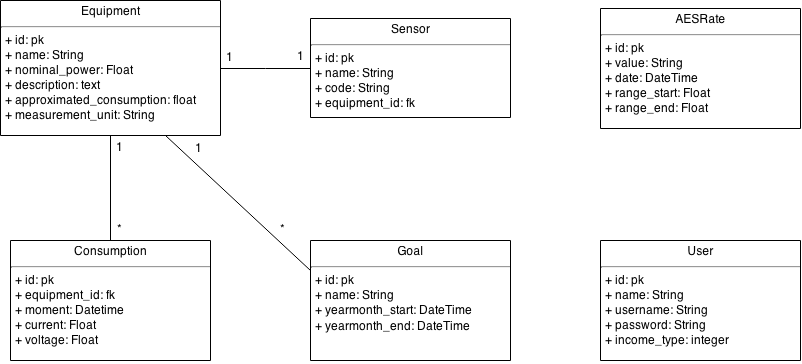
\includegraphics[width=1\textwidth]{figuras/diagrama_classes.png}
\caption{\label{fig:diagrama-classes} Diagrama de Classes}
\end{center}
\end{figure}

A seguir estão descritas as classes do sistema e seus atributos.

\subsubsection{Equipment}
\begin{description}
	\item[Classe:] Equipment
	\item[Descrição:] Representa um equipamento na aplicação. Os equipamentos são criados pelos usuários dentro do sistema. É necessário possuir um sensor associado para que o equipamento possa ser associado a um consumo.
	\item[Atributos:] \hfill
		\begin{enumerate}
		  \item id (integer): identificador do equipamento
		  \item name (String): nome do equipamento
		  \item description (Text): descrição do equipamento 
		  \item nominal\_power (float): potência nominal do equipamento 
		  \item measurement\_unit (String): unidade de medida utilizada em nominal\_power
		  \item approximated\_consumption (float): consumo aproximado do equipamento dado pelo fabricante 
		\end{enumerate}
	\item[Relacionamentos:] \hfill
		\begin{enumerate}
			\item um equipamento possui nenhum ou um sensor
			\item um equipamento possui nenhum ou vários consumos
			\item um equipamento possui nenhum ou várias metas
		\end{enumerate}
\end{description} 
%
\subsubsection{Sensor}
\begin{description}
	\item[Classe:] Sensor
	\item[Descrição:] Representa um sensor na aplicação. Os sensores são criados automaticamente pelo sistema ao receber um consumo de um sensor não registrado. O usuário poderá, então, editar o nome do sensor. Porém, como não há dado que indique em qual aparelho o sensor foi instalado, tal associação deve ser feita através de configuração (Caso de uso Configurar sistema). Caso um sensor seja alocado de um equipamento para outro, os novos consumos passarão a pertencer ao segundo equipamento.
	\item[Atributos:] \hfill
		\begin{enumerate}
			\item id (integer): identificador do sensor
			\item name (String): nome dado pelo usuário para o sensor
			\item code (String): identificador do sensor, enviada pelo módulo sensor (endereço MAC do XBee no módulo sensor)
			\item equipment\_id (integer): equipamento ao qual está associado
		\end{enumerate}
	\item[Relacionamentos:] \hfill
		\begin{enumerate}
			\item um sensor pertence a um ou nenhum equipamento
		\end{enumerate}
\end{description} 
%
\subsubsection{Consumption}
\begin{description}
	\item[Classe:] Consumption
	\item[Descrição:] Representa uma medida de consumo feita de um equipamento em um dado instante. Quando um consumo é enviado ao sistema, o valor da corrente, tensão e identificador do sensor são enviados. Caso o identificador do sensor não exista dentro do sistema, uma nova instância de sensor será criada. A partir do momento em que o sensor tiver um equipamento associado, consumos para aquele equipamento poderão ser criados. Caso um sensor seja alocado de um equipamento para outro, os consumos para o equipamento anterior vão continuar pertencendo ao mesmo, enquanto os novos consumos pertencerão ao segundo equipamento.
	\item[Atributos:] \hfill
		\begin{enumerate}
			\item id (integer): identificador do consumo
			\item equipment\_id (integer): identificador do equipamento
			\item moment (DateTime): a data e a hora de quando foi feita a medida
			\item current (float): corrente no momento da medida em amperes
			\item voltage (float): tensão da tomada do equipamento. 220V ou 127V
		\end{enumerate}
	\item[Relacionamentos:] \hfill
		\begin{enumerate}
			\item um consumo pertence a um equipamento
		\end{enumerate}
\end{description} 
%
\subsubsection{User}
\begin{description}
	\item[Classe:] User
	\item[Descrição:] Representa um usuário do sistema. 
	\item[Atributos:] \hfill
		\begin{enumerate}
			\item id (integer): identificador do usuário
			\item name (String):  nome do usuário
			\item username (String): nome de usuário usado para efetuar o login
			\item password (String encriptado): senha do usuário usada para efetuar o login
		    \item income\_type (String): o tipo de renda do usuário, Residencial ou Residencial de baixa renda, de acordo com a especificação da AES eletropaulo.
		\end{enumerate}
\end{description} 
%
\subsubsection{Goal}
\begin{description}
	\item[Classe:] Goal
	\item[Descrição:] Representa uma meta de consumo para um mês. Ao cadastrar a meta, ela calcula um valor igual a percentagem (value\_in\_percent) do total de consumo para um equipamento no mês anterior. Ao ser traçado o gráfico do mês pertencente ao da meta para aquele equipamento, um gráfico com o valor da meta será exibido.
	\item[Atributos:] \hfill
		\begin{enumerate}
			\item id (integer): identificador da meta
			\item equipment\_id (integer): identificador do equipamento
			\item name (String):  nome da meta
			\item value\_in\_percent (float): consumo pretendido em percentagem (em relação ao mês anterior)
			\item value\_absolute (float): consumo pretendido (em relação ao mês anterior)
			\item yearmonth\_start (DateTime): início do período da meta
		    \item yearmonth\_end (DateTime): fim do período da meta
		\end{enumerate}
	\item[Relacionamentos:] \hfill
		\begin{enumerate}
			\item uma meta pertence a um equipamento
		\end{enumerate}
\end{description} 
%
\subsubsection{AESRate}
\begin{description}
	\item[Classe:] AESRate
	\item[Descrição:] Representa a taxa de conversão da AES eletropaulo de kilowatts hora para reais. Esses valores são obtidos através da página de tarifas do site da AES Eletropaulo \cite{aes_site}. Caso o usuário queira visualizar o consumo em reais, o usuário deve escolher a opção de integrar o gráfico também (pois as tarifas são calculadas em função da energia consumida, e não em função potência consumida em dado instante). Em seguida, o sistema identifica qual taxa de conversão, dependendo da data do consumo (deve ser maior ou igual a valid\_date), tipo de renda (se é igual ao atributo name), faixa de consumo (o valor de consumo deve ser maior ou igual a range\_start e menor ou igual a range\_end). Identificada a taxa, o sistema multiplica o valor de cada ponto do gráfico com a soma de TE e TUSD da taxa para converter em reais.
	\item[Atributos:] \hfill
		\begin{enumerate}
			\item id (integer): identificador da taxa de conversão
			\item name (String): nome da taxa de conversão, o mesmo utilizado pela AES.
			\item te (float): tarifa de energia
			\item tusd (float): tarifa de uso do sistema de distribuição
			\item date (DateTime): o instante que a taxa de conversão foi buscada
			\item valid\_date (DateTime): data de início da validade das tarifas
			\item range\_start (float): o início da faixa de consumo que define a taxa de conversão
		    \item range\_end (float): o fim da faixa de consumo que define a taxa de conversão
		\end{enumerate}
\end{description} 